% =============================================================================

\vspace*{\fill}

\begin{figure}[!h]
\begin{lstlisting}[language=pseudo,style=block]
saes.v3.encs  rd, rs1, rs2, bs : v3.Proc(rd, rs1, rs2, bs, fwd=1, mix=0)
saes.v3.encsm rd, rs1, rs2, bs : v3.Proc(rd, rs1, rs2, bs, fwd=1, mix=1)
saes.v3.decs  rd, rs1, rs2, bs : v3.Proc(rd, rs1, rs2, bs, fwd=0, mix=0)
saes.v3.decsm rd, rs1, rs2, bs : v3.Proc(rd, rs1, rs2, bs, fwd=0, mix=1)
\end{lstlisting}
\caption{
  Instruction mnemonics, and their mapping onto pseudo-code functions, for \ISE{3}.
}
\label{fig:v3:mnemonics}
\end{figure}

\begin{figure}[!h]
\begin{lstlisting}[language=pseudo,style=block]
v3.Proc(rd, rs1, rs2, bs, fwd, mix):
  x     = AESSBox[rs2.8[bs]] if fwd else AESInvSBox[rs2.8[bs]]
  if   mix and  fwd: t1.32 = {GFMUL(x, 3),      x    ,      x   ,GFMUL(x, 2)}
  elif mix and !fwd: t1.32 = {GFMUL(x,11),GFMUL(x,13),GFMUL(x,9),GFMUL(x,14)}
  else             : t1.32 = {0, 0, 0, x}
  rd.32 = ROTL32(t1.32, 8*bs) ^ rs1
\end{lstlisting}
\caption{
  Instruction pseudo-code functions for \ISE{3}.
}
\label{fig:v3:pseudo}
\end{figure}

\begin{figure}[!h]
\begin{lstlisting}[language=pseudo,style=block]
lw              a0, 16(RK)      // Load Round Key
lw              a1, 20(RK)
lw              a2, 24(RK)
lw              a3, 28(RK)      // t0,t1,t2,t3 contains current round state.
saes.v3.encsm   a0, a0, t0, 0   // Next state for column 0.
saes.v3.encsm   a0, a0, t1, 1   // Current column 0 in t0.
saes.v3.encsm   a0, a0, t2, 2   // Next column 0 accumulates in a0
saes.v3.encsm   a0, a0, t3, 3
saes.v3.encsm   a1, a1, t1, 0   // Next state for column 1.
saes.v3.encsm   a1, a1, t2, 1
saes.v3.encsm   a1, a1, t3, 2
saes.v3.encsm   a1, a1, t0, 3
saes.v3.encsm   a2, a2, t2, 0   // Next state for column 2.
saes.v3.encsm   a2, a2, t3, 1
saes.v3.encsm   a2, a2, t0, 2
saes.v3.encsm   a2, a2, t1, 3
saes.v3.encsm   a3, a3, t3, 0   // Next state for column 3.
saes.v3.encsm   a3, a3, t0, 1
saes.v3.encsm   a3, a3, t1, 2
saes.v3.encsm   a3, a3, t2, 3   // a0,a1,a2,a3 contains new round state
\end{lstlisting}
\caption{
  An AES encryption round implemented using \ISE{3}.
}
\label{fig:v3:round}
\end{figure}

\vspace*{\fill}

% -----------------------------------------------------------------------------

\newpage

\vspace*{\fill}

\begin{figure}[!h]
\centering
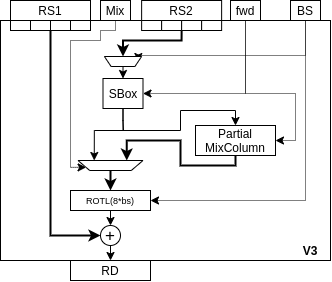
\includegraphics[width={0.5\textwidth}]{diagrams/ise-datapath-v3.png}
\caption{
  A diagramatic description of the functional unit required to support \ISE{3}.
}
\label{fig:v3:fu}
\end{figure}

\vspace*{\fill}

% =============================================================================
